\pdfminorversion=4
\documentclass[]{article}
\usepackage[utf8]{inputenc}
\usepackage{amssymb,latexsym,amsmath}
\usepackage[a4paper,top=3cm,bottom=2cm,left=3cm,right=3cm,marginparwidth=1.75cm]{geometry}
\usepackage{graphicx}
\usepackage[colorlinks=true, allcolors=blue]{hyperref}
\begin{document}

\title{Longest File Path using MapReduce}
\author{Dinh Khanh Minh Bi12-265}
\date{\today}

\maketitle

\tableofcontents
\newpage

\section{Introduction}
\subsection{Overview}
\noindent%
MapReduce is a programming model for distributed computing. It includes four main stages: splitting, mapping, shuffling, and reducing. Each stage is presented below:

\noindent%
- Splitting stage: Splitting is generally used during data processing in MapReduce programs. The input data is split equally based on user-defined. For example, a 100MB file can be split equally into four files; each file has a size of 25MB.

\noindent%
- Mapping stage: Each worker applies the map function to the data(usually in the file format). The mapper processes the data and creates several small chunks of data.

\noindent%
- Shuffling stage: Each worker nodes redistribute the data based on the output keys in a way such that all data with the same key belong to the same node

\noindent%
- Reducing stage: Each worker now processes the data after shuffling and produces the output


\subsection{Protocol}
\begin{figure}[h]
    \centering
    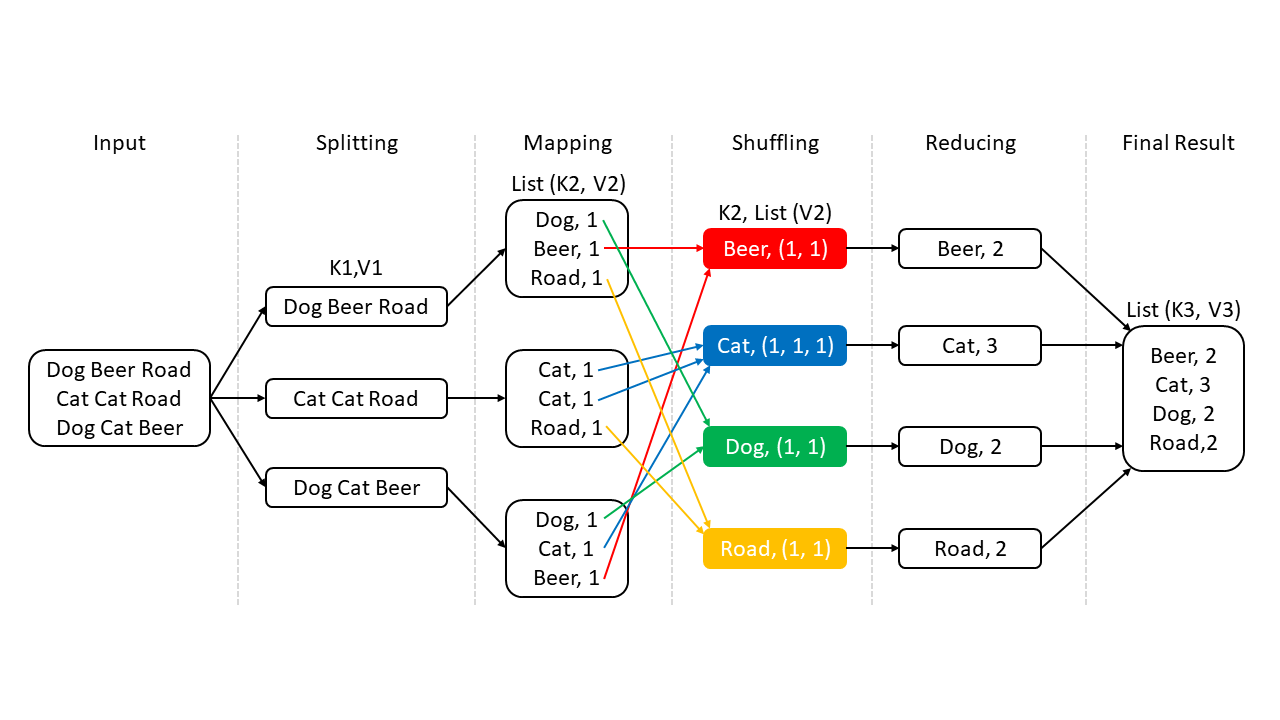
\includegraphics[scale=0.4]{images/mapreduce.png}
    \caption{MapReduce process\cite{MPI word count}}
    \label{fig:protocol}
\end{figure}

\subsection{Framework}
\noindent%
We use C in this project, so we have to implement the MapReduce framework ourselves.

\section{Methodology}
\begin{itemize}
    \item This code essentially recursively searches through a directory and its subdirectories to find the longest file path.
    \item Mapping and reducing follows the basic MapReduce pattern. 
    \item Afterwards, the server collects the results and print it out.
\end{itemize}

\section{Result}
\noindent%
This is the final result that we got:
\begin{figure}[h]
    \centering
    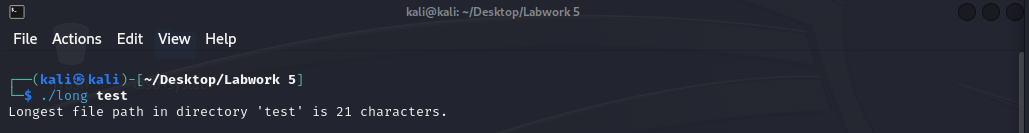
\includegraphics[scale=0.5]{images/results.PNG}
    \caption{Longest File Path program results}
    \label{fig:protocol}
\end{figure}

\begin{thebibliography}{9}
\bibitem{MPI word count}
https://www.oreilly.com/library/view/distributed-computing-in/9781787126992/5fef6ce5-20d7-4d7c-93eb-7e669d48c2b4.xhtml
\end{thebibliography}


\end{document}